% -*- latex -*-
% c3.tex
% LabSK 12.04.2022

% Wymagane pola (komentarz):
% Dawid Chmielewski				% Imię Nazwisko
% Praca w linii poleceń		% Temat ćwiczenia

\documentclass[a4paper,11pt]{article}

\usepackage[T1]{polski}
\usepackage[utf8]{inputenc}  			% Kodowanie pliku
\usepackage{pdfpages}

\hoffset=-3.0cm                         % Mniejszy lewy margines
\textwidth=18cm                         % szerzej
\evensidemargin=0pt

\voffset=-3cm                           % Mniejszy górny margines
\textheight=27cm                        % szerzej wzdłuż

\setlength{\parindent}{0pt}             % Paragraf od początku linii
\setlength{\parskip}{\medskipamount}    % Odstęp pomiędzy paragrafami
\raggedbottom                           % bez rozciągania strony

% Dodatkowe komendy
\newcommand\BS{\char`\\}                % \BS == back-slash
\newcommand\TY{\raise.17ex\hbox{$\scriptstyle\mathtt{\sim}$}}   % \TY == większa tylda w \tt

\thispagestyle{empty}			        % bez numeracji stron
\usepackage{enumerate}

\begin{document}
\title{ Sieci komputerowe - sprawozdanie }
\author{ Dawid Chmielewski, numer indeksu: 311188 }
\date{12 kwietnia 2022}

\maketitle{Temat ćwiczenia: Konfiguracja środowiska. Diagnostyka adresów IP.}

\section{Ogólny cel ćwiczenia}

Ćwiczenie obejmowało połączenie dwóch komputerów za pomocą samodzielnie zaprojektowanej sieci, wliczając w to konfigurację interfejsów i obserwację ruchu sieciowego, a także podłączenie dysku LabSK do maszyny domowej.

\section{Podłączenie dysku LabSK do maszyny domowej}

Dzięki podpięciu dysku LabSK mam do niego szybki i prosty dostęp jako do klikalnego katalogu z eksploratora plików. Aby to zrealizować, odnalazłem plik {\tt hosts} pod pełną ścieżką:

{\tt
\begin{verbatim}
    C:\Windows\System32\drivers\etc
\end{verbatim}
}

Konieczna była jego edycja, czyli dodanie na koniec tego pliku linii z odpowiednim adresem:

{\tt
\begin{verbatim}
    10.146.146.22   ftp     # Server LabSK na PW
\end{verbatim}
}

Po zapisaniu zmian sprawdziłem połączenie poleceniem {\tt ping}.

{\tt
\begin{verbatim}
    PS C:\Users\Dawid> ping ftp -n 1

    Pinging ftp [10.146.146.22] with 32 bytes of data:
    Reply from 10.146.146.22: bytes=32 time=1ms TTL=64

    Ping statistics for 10.146.146.22:
        Packets: Sent = 1, Received = 1, Lost = 0 (0% loss),
    Approximate round trip times in milli-seconds:
        Minimum = 1ms, Maximum = 1ms, Average = 1ms
\end{verbatim}
}

Od tej pory mam prosty dostęp do zasobów dysku z przydatnymi materiałami do zajęć. Wystarczy, że w eksploratorze plików, w pasku zadań wpiszę {\tt \begin{verbatim} \\ftp \end{verbatim}} i wprowadzę stosowne dane do logowania: login {\tt stud} i hasło {\tt zetis}.

\section{Zaprojektowanie własnej sieci}

\subsection{Diagram sieci}

Swoją sieć zaprojektowałem zgodnie z poniższym diagramem. Wybrałem stacje {\tt s8} oraz {\tt s4}. Adres to {\tt 10.64.63.0/24} - czyli maska 24-bitowa.

Projekt jest widoczny poniżej:

\pagebreak
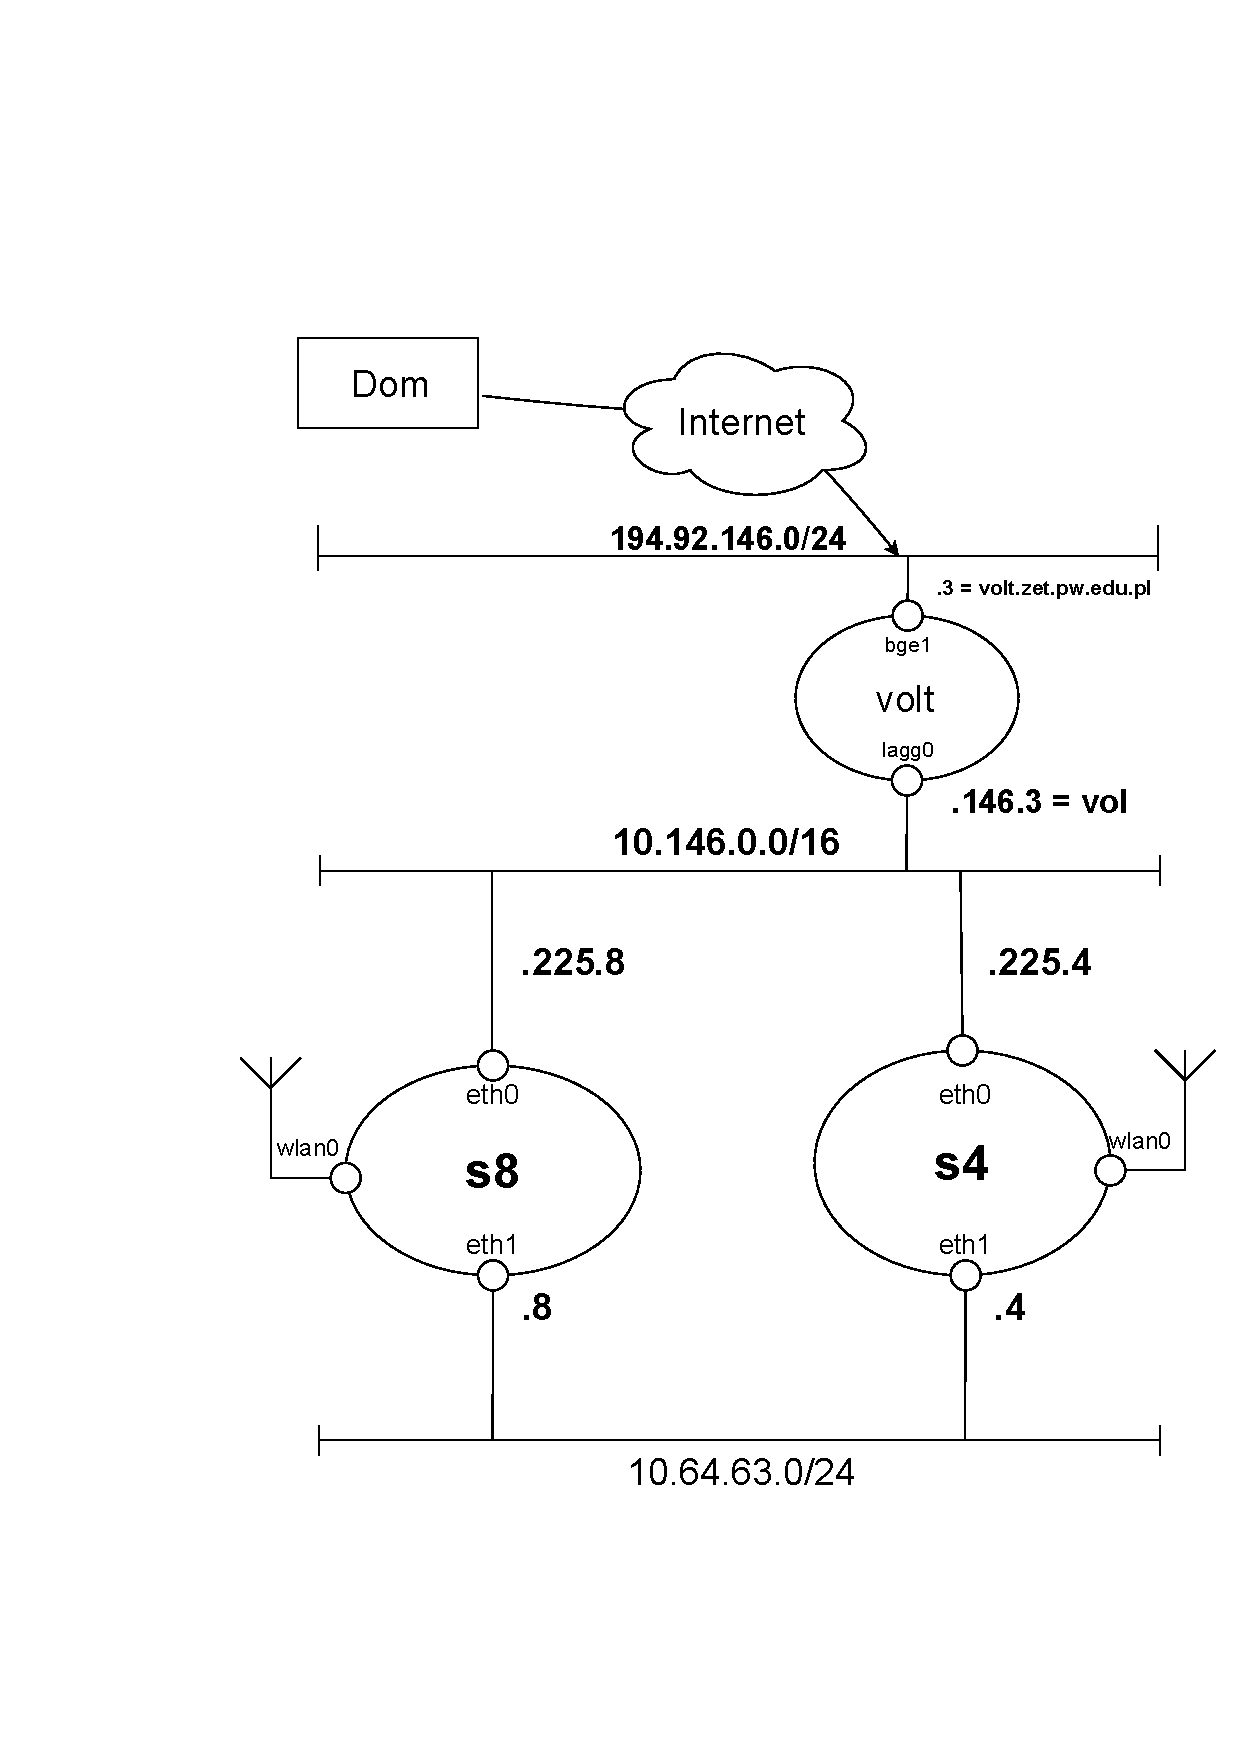
\includepdf[pages=-]{siec_drawio.pdf}

\subsection{Konfiguracja adresów IP} 

Wylistowanie interfejsów:

{\tt
\begin{verbatim}
    stud@archiso ~ % ip -br a
    lo               UNKNOWN        127.0.0.1/8 ::1/128
    eth0             UP             10.146.225.8/16 fe80::24e1:e7da:56c6:6ef8/64
    eth1             UP             10.146.90.11/16 fe80::a31e:94d2:7c87:13ce/64
    wlan0            DOWN
    stud@archiso ~ % sudo ip address add 10.64.63.8/24 dev eth1
\end{verbatim}
}

Interfejs, który mnie interesuje, nazywa się {\tt eth1}. W związku z tym, musiałem dodać na maszynach odpowiednie adresy oraz usunąć poprzednie.
Na stacji {\tt s4} konfiguracja wyglądała następująco:
{\tt
\begin{verbatim}
    stud@archiso ~ % sudo ip address add 10.64.63.4/24 dev eth1
    stud@archiso ~ % sudo ip address del 172.29.225.4/16 dev eth1
    stud@archiso ~ % ip -br a
    lo               UNKNOWN        127.0.0.1/8 ::1/128
    eth0             UP             10.146.225.4/16 fe80::2754:6710:5c2b:ebae/64
    eth1             UP             10.64.63.4/24 fe80::de2d:a5ce:cd7c:f592/64
    wlan0            DOWN
\end{verbatim}
}

Jak widać, na interfejsie {\tt eth1} udało mi się zmienić adres IP na zgodny z moim projektem. Dla stacji s8 konfiguracja wyglądała analogicznie.

{\tt
\begin{verbatim}
    stud@archiso ~ % sudo ip address add 10.64.63.8/24 dev eth1
    stud@archiso ~ % sudo ip address del 10.146.90.11/16 dev eth1
    stud@archiso ~ % ip -br a
    lo               UNKNOWN        127.0.0.1/8 ::1/128
    eth0             UP             10.146.225.8/16 fe80::24e1:e7da:56c6:6ef8/64
    eth1             UP             10.64.63.8/24 fe80::a31e:94d2:7c87:13ce/64
    wlan0            DOWN
\end{verbatim}
}

\subsection{Sprawdzenie połączenia między maszynami}

Polecenie {\tt ping} pozwoliło mi sprawdzić, czy połączenie rzeczywiście działa- sprawdziłem to dla każdej z obu stacji.
Dla stacji {\tt s8}, sprawdzając połączenie z {\tt s4}:

{\tt
\begin{verbatim}
    1 stud@archiso ~ % ping -c1 10.64.63.4
    PING 10.64.63.4 (10.64.63.4) 56(84) bytes of data.
    64 bytes from 10.64.63.4: icmp_seq=1 ttl=64 time=0.237 ms
    
    --- 10.64.63.4 ping statistics ---
    1 packets transmitted, 1 received, 0% packet loss, time 0ms
    rtt min/avg/max/mdev = 0.237/0.237/0.237/0.000 ms
\end{verbatim}
}

Dla stacji {\tt s4}, sprawdzając połączenie z {\tt s8}:

{\tt
\begin{verbatim}
    stud@archiso ~ % ping 10.64.63.8
    PING 10.64.63.8 (10.64.63.8) 56(84) bytes of data.
    64 bytes from 10.64.63.8: icmp_seq=1 ttl=64 time=0.246 ms
    (...)
    --- 10.64.63.8 ping statistics ---
    5 packets transmitted, 5 received, 0% packet loss, time 4064ms
    rtt min/avg/max/mdev = 0.232/0.241/0.246/0.005 ms
\end{verbatim}
}

\subsection{Analiza ruchów sieciowych}

Analiza ruchów sieciowych jest możliwa za pomocą tcpdump. Użyłem go na stacji {\tt s8}, a na {\tt s4} użyłem polecenia ping:

{\tt
\begin{verbatim}
    stud@s4 ~ % ping -c1 10.64.63.8
\end{verbatim}
}

{\tt
\begin{verbatim}
    stud@s8 ~ % sudo tcpdump -i eth1 icmp
    tcpdump: verbose output suppressed, use -v[v]... for full protocol decode
    listening on eth1, link-type EN10MB (Ethernet), snapshot length 262144 bytes
    00:11:25.215214 IP s8 > s4: ICMP echo reply, id 17, seq 1, length 64

    1 packet captured
    5 packets received by filter
    0 packets dropped by kernel 
\end{verbatim}
}

{\tt
\begin{verbatim}
    stud@s8 ~ % sudo tcpdump -i eth1 icmp
    tcpdump: verbose output suppressed, use -v[v]... for full protocol decode
    listening on eth1, link-type EN10MB (Ethernet), snapshot length 262144 bytes

    00:13:10.397633 IP s8 > s4: ICMP echo reply, id 18, seq 1, length 64

    1 packet captured
    1 packet received by filter
    0 packets dropped by kernel 
\end{verbatim}
}

\end{document}